\documentclass{scrartcl}
\usepackage[top=3cm, bottom=3cm, left=2cm,right=2cm]{geometry} 

\usepackage[english]{babel}
\usepackage[utf8]{inputenc}
\usepackage{mathtools}
\usepackage{esvect}
\usepackage{amssymb}
\usepackage{amsmath}

\usepackage{dcolumn}
\usepackage{booktabs}
\usepackage{tikz}
\usepackage{graphicx}
\usepackage{multicol}
\usepackage{float}
\usepackage{url}

\usepackage{listings}

\usepackage[toc, page]{appendix}


\DeclareMathOperator*{\argmin}{argmin} % no space, limits underneath in displays
\DeclareMathOperator*{\argmax}{argmax} % no space, limits underneath in displays

\DeclarePairedDelimiter\abs{\lvert}{\rvert}%
\DeclarePairedDelimiter\norm{\lVert}{\rVert}%

\usepackage{titlesec}
\newcommand{\sectionbreak}{\clearpage}

\usepackage[parfill]{parskip}
\parskip = 4pt

\title{FoundCrypt - Summary}
\author{Sebastian Rietsch}

\begin{document}
\maketitle
\tableofcontents

\section{Part 1: Reasoning About Distributed Systems Models and Algorithms}
A distributed system consists of:
\begin{itemize}
    \item
        a finite set of sequential processes (or processors, agents, threads)
    \item
        a communication system (typically using messages)
\end{itemize}
Many things to consider: State changes within processes can take place concurrently, communication is unreliable and costly, local failures can happen, ...

\begin{figure}
    \begin{center}
        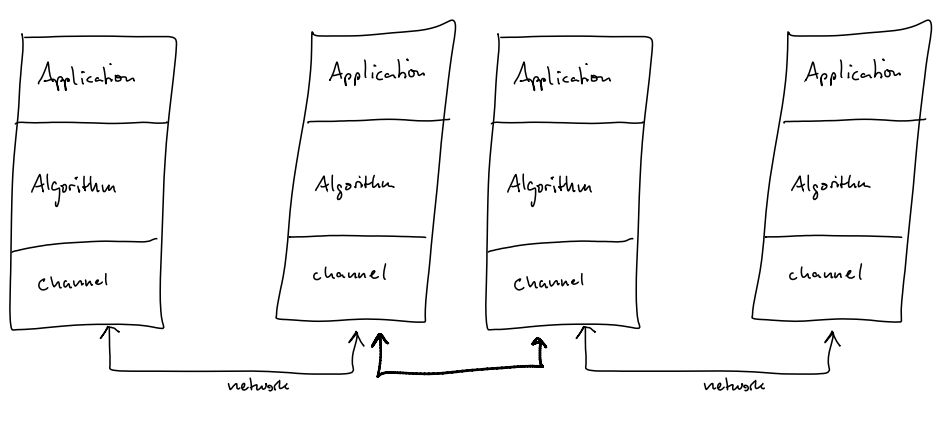
\includegraphics[scale=0.5]{img/distsys}
        \caption{Structure of Distributed Systems}
    \end{center}
\end{figure}

\bigbreak

The application needs underlying services for many-to-many interaction: reliability guarantees are only offered for pairs of processes, i.e. one-to-one communication.

\(\Rightarrow\) Reliable broadcast: Ensure that a mesage which is sent by one process is received by all other processes (or none)

\subsection{Formalizing distributed algorithms}
\textbf{Channels} (abstracting networks)

 \textbf{Processes} (abstracting computers):
\begin{itemize}
    \item
        Each process has local clock
    \item
        At each clock tick a process executes a step, which consists of:
        \begin{enumerate}
            \item
                A local computation (local event) and
            \item
                message exchanges with other processes (global event)
        \end{enumerate}
    \item
        Assumption: at most one message is delivered from or sent to a process per step
\end{itemize}

\bigbreak

\textbf{Software Stack}:
\begin{itemize}
    \item
        A processes program is made of a finite set of modules organized as a stack
    \item
        Modules within the same process interact by exchanging event (with attributes)
    \item
        Between every module there is a local event queue, they get processed in FIFO order
    \item
        Three types of events:
        \begin{enumerate}
            \item 
                \textbf{Request}: request aservice from a lower layer
            \item
                \textbf{Confirmation}: confirm that request has been received/executed
            \item
                \textbf{Indication}: indicate that something has happend, e.g., a message which was broadcast is delivered
        \end{enumerate}
\end{itemize}

\textbf{Example: Reliable Broadcast}
\begin{itemize}
    \item
        Interface for the \textbf{application}:
        \begin{itemize}
            \item
                broadcast(m): request event
            \item
                deliver(m): indication event
        \end{itemize}
    \item
        Interface used by the \textbf{algorithm}:
        \begin{itemize}
            \item
                send(m, p): request event
            \item
                receive(m, q): indication event
        \end{itemize}
\end{itemize}

\section{Part 2: Modeling Distributed Systems}
\subsection{Specification}
\begin{itemize}
    \item
        The \textbf{interface} of a software module is given by the \textbf{types of events} which may occur 
    \item
        The \textbf{properties} of a software module at its interface
        \begin{itemize}
            \item
                What events are (not) assumed to happen?
            \item
                What events should eventually happen?
        \end{itemize}
    \item
        Should be as precise as possible
\end{itemize}
\subsubsection{Liveness and Safety}
\textbf{Safety:}
\begin{itemize}
    \item
        States that something bad never happens    
    \item
        Characterized by some "irremedial" bad event (can't be made good again)
    \item
        "It is never the case that ..."
    \item
        Are \textbf{violated} in finite time, can be observed
    \item
        Are \textbf{satisifed} in infinite time (to witness, you have to live forever) 
\end{itemize}

\textbf{Liveness:}
\begin{itemize}
    \item
        States that something good should happen eventually
    \item
        Characterized by the fact that no event can really violate them
    \item
        "Eventually...", "Whenever ... then eventually..."
    \item
        Are \textbf{violated} in infinite time, e.g. when the algorithm never terminates
    \item
        Are \textbf{satisfied} in finite time, e.g. when the algorithm terminates
\end{itemize}

\bigbreak

To check, if property \(P\) is a safety or liveness property, ask:
\begin{itemize}
    \item
        Is there a finite point in time where I can observe \textbf{at the interface} that \(P\) is violated?
    \item
        Answer yes \(\Leftrightarrow\) \(P\) is safety property
\end{itemize}

\subsubsection{Weak Best-Effort Broadcast}
Interface:
\begin{itemize}
    \item
        Request: wbebBroadcast(m)
    \item
        Indication: wbebDeliver(src, m)
\end{itemize}

Properties:
\begin{itemize}
    \item
        If \(p\) and \(q\) do not fail then every message broadcast by \(p\) will eventually be delivered by \(q\) (Liveness)
    \item
        No message is delivered unless it was broadcast (Safety)
\end{itemize}

\subsection{Assumptions about processes, channels, and their failures}
We look at \textbf{fault assumptions} or \textbf{failure models} here.
\subsubsection{Processes}
\begin{itemize}
    \item
        A process either executes the algorithm assigned to it or fails 
    \item
        We only consider \textbf{Crash-Stop:}
        \begin{itemize}
            \item
                A process simply stops to execute steps
            \item
                It does not send or receive any messages anymore
        \end{itemize}
    \item
        Terminology:
        \begin{itemize}
            \item
                A \textbf{correct process} is a process that does not fail
            \item
                A \textbf{faulty process} is a process which is not correct
                
        \end{itemize}
\end{itemize}

\subsubsection{Channels}
\textbf{Fair-loss Link}: if you try often enough, eventually the message will get through and messages don't appear out of nowhere
Formally:
\begin{itemize}
    \item
        \textbf{FL1} (Fair-Loss): If a message \(m\) is sent infinitely often by \(p_i\) and neither \(p_i\) or \(p_j\) crash, then \(m\) is delivered infinitely often to \(p_j\) 
    \item
        \textbf{FL2} (Finite duplication): If a message is sent a finite number of times by \(p_i\) to \(p_j\), it is delivered a finite number of times by \(p_j\)
    \item
        \textbf{FL3} (No creation): No message is delivered unless it was sent
\end{itemize}

\textbf{Interface:}
\begin{itemize}
    \item
        flp2pSend
    \item
        flp2pDeliver
\end{itemize}

\subsection{Example: Building perfect communication links}
\subsubsection{Stubborn links from fair-loss links}
\textbf{Specification:}
\begin{itemize}
    \item
        \textbf{SL1} (Stubborn delivery): if a process \(p_i\) sends a message \(m\) to a correct process \(p_j\), and \(p_i\) does not crash, then \(p_j\) delivers \(m\) an infinite number of times 
    \item
        \textbf{SL2} (No creation): No message is delivered unless it was sent
\end{itemize}

\textbf{Interface:}
\begin{itemize}
    \item
        sp2pSend
    \item
        sp2pDeliver
\end{itemize}

\textbf{Algorithm (sl)}:
\begin{lstlisting}
upon event <sp2pSend, dest, m> do
    while(true) do
        trigger <flp2pSend, dest, m>;

upon event <flp2pDeliver, src, m> do
    trigger <sp2pDeliver, src, m>;
\end{lstlisting}

\subsubsection{Reliable (perfect) links from stubborn links}
\textbf{Specification}:
\begin{itemize}
    \item
        \textbf{PL1} (Validity): If \(p_i\) and \(p_j\) are correct, then every message sent by \(p_i\) to \(p_j\) is eventually delivered by \(p_j\)  
    \item
        \textbf{PL2} (No duplication): No message is deliveres (to a process) more than once
    \item
        \textbf{PL3} (No creation): No message is delivered unless it was sent
\end{itemize}

\textbf{Algorithm} (pl):
\begin{lstlisting}
upon event <Init> do delivered := empty;

upon event <pp2pSend, dest, m> do
    trigger <sp2pSend, dest, m>;

upon event <sp2pDeliver, src, m> do
    if m not in delivered then
        trigger <pp2pDeliver, src, m>;
        add m to delivered;
\end{lstlisting}

\subsection{Assumptions about timing}
\end{document}
